\chapter{Methods and Theoretical Background}

This chapter explains the methods, discusses the underlying theory, and outlines key assumptions. 

\section{Benford's Law Formulation}

The relative frequency of a leading digit approaches 

\begin{equation}
    \label{BZ-general_first}
\text{P(} X = d_i\text{)}= \log_{10}(1+1/d_i)
\end{equation}

where $d_i \in \{1,\dots,9\}$ for first digit law and $d_i \in \{10,\dots,99\}$ for the first-two digits law or even $d_i \in \{100,\dots,999\}$ for the first-three digits law. For other values (negative $d_i$) the probability is 0. When plotted, it resembles nice logarithmic distribution, as seen on figure \ref{fig:FL}.  \cite{Cerqueti2202,Hronova2023,Newcomb1881}

\begin{figure}[h]
    \centering
    \caption{Theoretical frequencies of the first leading digits}
    \label{fig:FL}
    \pgfplotsset{width=8.5cm,compat=1.18}
        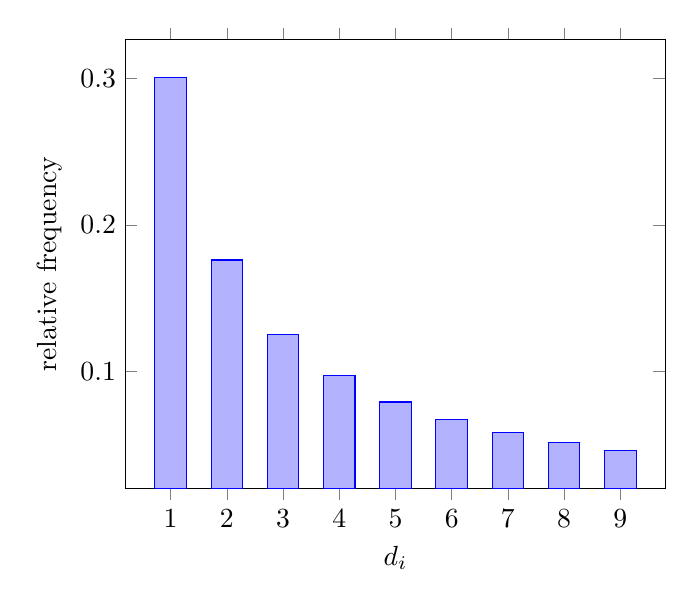
\begin{tikzpicture}
        \definecolor{clr1}{RGB}{00,152,129} 
            \begin{axis}[
                ybar,
                bar width=.4cm,
                enlargelimits=0.1,
                ylabel={relative frequency},
                xlabel={$d_i$},
                symbolic x coords={1,2,3,4,5,6,7,8,9},
                xtick=data,
                ]
            \addplot coordinates {(1,0.3010) (2,0.1761) (3, 0.1249) (4,0.0969) (5,0.0791) (6,0.0669) (7,0.0580) (8,0.0512) (9,0.0458)};
            \end{axis}
        \end{tikzpicture}
    \source{ and processing: author}
\end{figure}

The first leading digit is the one found at the highest order and is non-zero. In the case of the number 124.857, the first digit would be 1, whereas for the number 0.03958, the first digit would be 3. According to Benford's law of the first digit, the theoretical frequencies correspond to the equation \ref{BZ-general_first}, indicating that the digit 1 occurs in the first position with a probability of 0.3, the digit 2 with 0.18, and so forth, with the digit 9 occurring with a probability of only 0.046. For all first digits from 1 to 9, see the BL column in the table in the Figure \ref{table:BL-table}.
%Compliance to this distribution is the first step in the nine-step procedure recommended by \citeauthor{kossovsky2014benford}, as mentioned in section \ref{correct_usage}.

As can be seen in the graph \ref{fig:FL}, the distribution is heavily skewed in favour of the lowest digits. As we move to the second (figure \ref{fig:second-digit-law}) and higher digits, this skew will flatten out significantly until there is no difference between the digits.  \cite{kossovsky2014benford}

This can be described by 

\begin{equation}
    \label{BZ-general_second}
    P(d) = \sum\limits_{k=1}^{9} \log_{10}\left( 1+\frac{1}{10k+d}\right), \quad \text{for } d = 0,1,\dots,9
\end{equation}

as mentioned by \citeauthor{Hronova2023} in \citeyear{Hronova2023}, assuming the independent occurence of the second leading digits. 

\begin{figure}[h]
    \centering
    \caption{Theoretical frequencies of the second leading digits}  
    \label{fig:second-digit-law}
        \pgfplotsset{width=8.5cm,compat=1.18}
            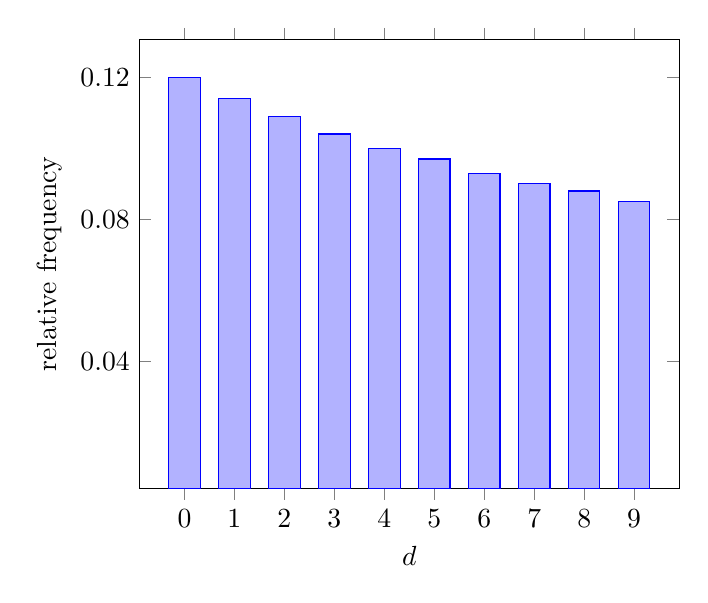
\begin{tikzpicture}
            \definecolor{clr1}{RGB}{00,152,129} 
                \begin{axis}[
                    ybar,
                    bar width=.4cm,
                    ymin=0.015,
                    ytick={0.12, 0.08, 0.04},
                    enlargelimits=0.1,
                    ylabel={relative frequency},
                    xlabel={$d$},
                    symbolic x coords={0, 1,2,3,4,5,6,7,8,9},
                    xtick=data,
                    yticklabel style={/pgf/number format/fixed, /pgf/number format/precision=2},
                    ]
                \addplot coordinates {(0,0.12) (1,0.114) (2,0.109) (3, 0.104) (4,0.10) (5,0.097) (6,0.093) (7,0.09) (8,0.088) (9,0.085)}; %[clr1,fill=clr1,opacity=0.55]
                \end{axis}
            \end{tikzpicture}
    \source{ and processing: author}
\end{figure}

The distribution for the second digits is less skewed than that of the first leading digits. 
%Compliance to this distribution is the second step in the nine-step procedure recommended by \citeauthor{kossovsky2014benford}, as mentioned in section \ref{correct_usage}.
Coming to the third leading digit, the relative frequencies start to be close to equal as seen on figure \ref{fig:third-digit-law}. \cite{kossovsky2014benford}

This is explained by the following equation 

\begin{equation}
    P(d) = \sum\limits_{d_1=1}^{9} \sum\limits_{d_2=1}^{9} \dots \sum\limits_{d_{k-1}=1}^{9}   \log_{10}\left( 1+\frac{1}{\sum\limits_{i=1}^{k} d_i \cdot 10^{k-i} }\right), \quad \text{for } d_k = 0,1,\dots,9 
\end{equation}

describing third and following position relative frequencies, again with the assumption of independence of digit occurrences. And \uv{\emph{the Benford distribution converges to a uniform
multinomial distribution}} as put in \citeauthor{Hronova2023} in \citeyear{Hronova2023}. 

\begin{figure}[ht!]
    \centering
    \caption{Theoretical frequencies of the third leading digits}  
    \label{fig:third-digit-law}
    \pgfplotsset{width=8.5cm,compat=1.18}
        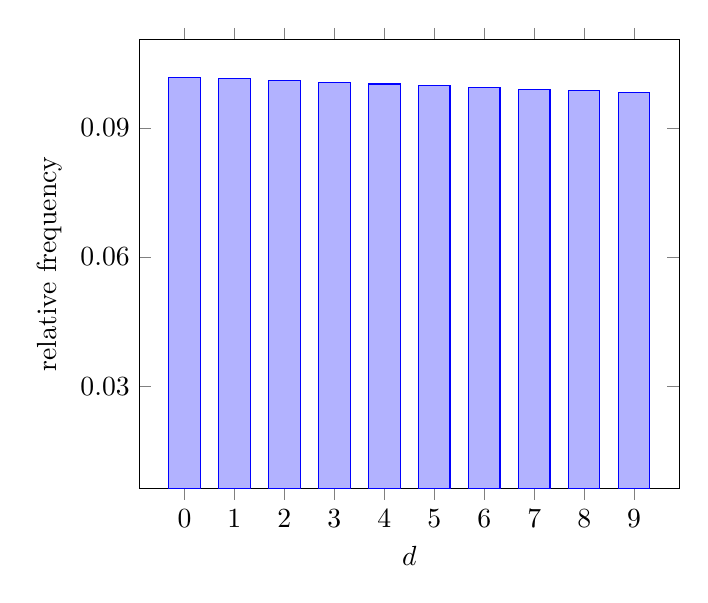
\begin{tikzpicture}
        \definecolor{clr1}{RGB}{00,152,129} 
            \begin{axis}[
                ybar,
                bar width=.4cm,
                ymin=0.015,
                ytick={0.09, 0.06, 0.03},
                enlargelimits=0.1,
                ylabel={relative frequency},
                xlabel={$d$},
                symbolic x coords={0,1,2,3,4,5,6,7,8,9},
                xtick=data,
                yticklabel style={/pgf/number format/fixed, /pgf/number format/precision=2},
                ]
            \addplot coordinates {(0,0.1018) (1,0.1014) (2,0.1010) (3, 0.1006) (4,0.1002) (5,0.0998) (6,0.0994) (7,0.0990) (8,0.0986) (9,0.0983)};
            
            \end{axis}
        \end{tikzpicture}
    \source{ and processing: author}
\end{figure}

So for digits in the last position, the distribution is expected to be very close to, if not uniform. 


\subsection{Uniform discrete distribution}

Distribution, where every value of a random discrete variable $X$ has the same probability, is named the uniform distribution. It has many uses, eg., can be used to select a value from a set, when all values have the same probability. The probability is 

\begin{equation}
\begin{aligned}
    P(d) &= \frac{1}{n}, &\qquad d=0,1,\dots,n \\
         &= 0,           &\qquad \text{else.}
\end{aligned}
\end{equation}


If digits in a long enough number were distributed equally, according to the uniform distribution, the distribution would look like in figure \ref{fig:BZ-uniform}, where all digits have the probability of 0.1. \cite{kossovsky2014benford, Hronova2023, Marek2024}

\begin{figure}[ht!]
    \centering
    \caption{Theoretical frequencies of digits under uniform distribution}  
    \label{fig:BZ-uniform}
    \pgfplotsset{width=8.5cm,compat=1.18}
        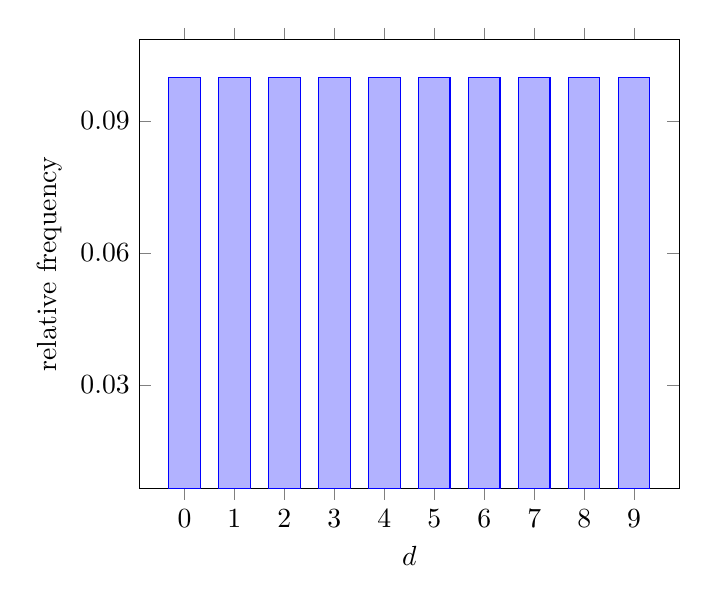
\begin{tikzpicture}
        \definecolor{clr1}{RGB}{00,152,129} 
            \begin{axis}[
                ybar,
                bar width=.4cm,
                ymin=0.015,
                ytick={0.09, 0.06, 0.03},
                enlargelimits=0.1,
                ylabel={relative frequency},
                xlabel={$d$},
                symbolic x coords={0,1,2,3,4,5,6,7,8,9},
                xtick=data,
                yticklabel style={/pgf/number format/fixed, /pgf/number format/precision=2},
                ]
            \addplot coordinates {(0,0.1) (1,0.1) (2,0.1) (3, 0.1) (4,0.1) (5,0.1) (6,0.1) (7,0.1) (8,0.1) (9,0.1)};
            \end{axis}
        \end{tikzpicture}
    \source{ and processing: author}
\end{figure}

\subsection{The Scale Invariance Principle of Benford's Law}

Given a dataset that behaves according to BL, changing units (multiplying the whole dataset by the same constant) will still behave according to BL. Any arithmetic operation applied to the whole dataset does not change the underlying BL distribution. \cite{kossovsky2014benford, Hronova2023} %section 23 The Scale Invariance Principle 

\subsection{Digital Development Pattern} \label{DDPattern}

Digital development pattern refers to the way distributions of digits evolve across different ranges of data. This pattern is observed in all random data sets, whether they follow Benford's Law or not. The pattern shows how the distribution of digits changes from lower to higher values of the data range. 

This pattern can only be seen when the data range is partitioned along integral powers of ten, such as (0.1, 1), (1, 10), (10, 100), etc. The pattern shows increasing skewness as you move from the left to the right of the data range. For smaller values, digit distributions are more equal. In the centre, the distribution becomes more logarithmic. For larger values, the distribution becomes highly skewed in favour of low digits. \cite{kossovsky2014benford}


\subsection{Applicability of Benford's Law}

The law does not impose many conditions on the data that will be analysed, yet some must be met for reliable results. This section will discuss the following. 

\subsubsection*{Order of Magnitude of Variability (OMV)}

\citeauthor{kossovsky2014benford} notes that for data to behave according to BL, its value range should be wider, rather than narrow. He describes a measure, Order of Magnitude of Variability (OMV), as 

\begin{equation}
    OMV = \log_{10}(\text{90th percentile}) - \log(\text{10th percentile}) > 3 
    \label{OMV}
\end{equation}

and recommends it should be larger than 3. In practice, this means that our data should spread all the way from 1 to 10000 or more for consistent results. If we were to use data with lower OMV than recommended, we would get results that look fraudulent, while being genuine - data like this has higher probabilities of type I error when testing for compliance with BL.

However, election data, analysed in this thesis, should comply with the BL distribution either way. For our purposes, we will focus on a more liberal measure, the Order of Magnitude OOM, that is defined as

\begin{equation}
    OOM = \log_{10}(\text{max}) - \log(\text{min}) > 3. 
    \label{OOM}
\end{equation}

This measure works best when outliers are removed. When rejected, the convergence of BL to the uniform distribution is flawed and specific frequencies for digits on given positions should rather be used. \cite{kossovsky2014benford}
 
\subsubsection*{Correct usage} 

The compliance of our data with the law can be expected when only minimal conditions are met. Then the conformity can be tested. This makes the law good for detecting the presence of fraud or various manual manipulations of numbers with high accuracy. \cite{kossovsky2014benford, Cerqueti2202,kossovsky2014benford} 

When using Benford's Law to detect intentional fraud or data manipulation, the complete dataset is used, rather than a subset. Additionally, the dataset must satisfy conditions other than those mentioned in the previous chapters. The dataset should be large enough - for datasets with less than 100 observations, BL analysis is not recommended. %\cite{kossovsky2014benford} % section 26, strana 82
Only non-negative data should be used for analysis. For use in auditing, it is also recommended to eliminate small numbers, values less than, for example, 50, but that the portion removed be less than $10\%$. In addition, values that represent totals, summations, etc., should not be included if they come from the same sample. \cite{kossovsky2014benford} % section 27, strana 88 

\subsubsection*{Varying results from the expected distribution}

It is generally advisable to focus on deviations from the theoretical distribution in a given BL variation, specifically on the significantly higher values for the frequency of occurrence of a given digit. In graphical representation, these can be represented as spikes. There is minimal interest in the reduced frequencies, as any suspicious activity is likely to manifest itself through increased frequencies - when counting frequencies, an increase in one digit is much more detectable, with all other frequencies dropping slightly. \cite{kossovsky2014benford} % section 26, strana 85 

% \begin{koment}
%     grafický příklad jak vypadá hrot jakožto odchylka od konformity s BZ - pokud nebudu mít nic svého, Kossovsky strana 83. Potom i další ukázky podivných situací.
% \end{koment}

%There will always be variation, because few datasets are $100\%$ \textit{Benfordian}.  \cite{kossovsky2014benford} % section 26, strana 84

Deviance is to be expected, but where should the line be drawn?  \citeauthor{kossovsky2014benford} suggests distinguishing between two terms: compliance and comparison. When researching the data's compliance with BL, the data is expected to follow the logarithmic distribution very closely, the focus is on detecting manipulation, and if there is, whether it is random or structural. For our use, we assume the data follows the distribution and therefore observe data compliance.

Next, the deviations should not show signs of any systematic error or pattern. Some pattern may emerge by rounding numbers, for example. The practice of rounding data is prevalent in the context of accounting, where values ending in 00 or 50 are frequently observed. This rounding process, which is often employed to streamline computations, can give rise to manipulation of higher orders while being harmless in context. Empirical evidence supports the prevalence of these values in practice. 
However, such manipulations are unacceptable in, for example, electoral statistics, where votes simply cannot be rounded.
\cite{kossovsky2014benford} %\cite{kossovsky2014benford} %section 27, strana 92

Alternatively, the validity of BL can be influenced by changed external situations in regards to the data itself. For instance, how does sales data follow BL distribution when affected by the pandemic in 2020? This has been answered by \citeauthor{Hronova2023} in \citeyear{Hronova2023}. Changes like this should be taken into account, and analysis should be adapted accordingly.


% \section{Descriptive statistics}

% % \subsection{Miry polohy}

% \subsection{Expected value}

% For discrete variables: 
% \begin{equation}
%     % E(X) = \frac{1}{n} \sum \limits_{i=0}^{n} X_i
%     E(X) = \sum \limits_{i=0}^{n} x_i P(X=x_i)
% \end{equation}

% For continuos variables: 
% \begin{equation}
%     % E(X) = \frac{1}{n} \sum \limits_{i=0}^{n} X_i
%     E(X) =  \int \limits_{-\infty}^{\infty} x f(x) dx
% \end{equation}

% \cite{Marek2024} 

% % \subsection{Miry variability}

% \subsection{Variance}

% Variance is a measure of variability, its square root is the standard deviation. 

% \begin{equation}
%     D(X) = E(X^2) - E(X)^2 = E\{[X-E(X)]^2\}
% \end{equation}

% \begin{equation}
%     \text{sd}(X) = \sqrt{D(X)} 
% \end{equation}

% \cite{Marek2024}


% \subsection{Correlation}

% Correlation or correlation coefficient describes the relationship or dependency between two variables. It is defined as 

% \begin{equation}
%     \rho(X,Y) = \frac{\text{cov}(X,Y)}{\sqrt{D(X)D(Y)}} 
% \end{equation}

% and cov$(X,Y)$ is covariance and is defined as: 

% \begin{equation}
%  \text{cov}(X,Y) = E(X-E(X), Y-E(Y)) = E(XY)-E(X)E(Y). 
% \end{equation}

% Covariance and correlation both contain the same information, but the correlation coefficient in a given range: $\rho(X,Y) \in \langle-1,1\rangle$. The value -1 denotes a very strong negative dependency of X and Y variables, 0 is no relationship and 1 is a strong positive dependency of the variables. 

% \cite{Marek2024}

\section{Selected relevant distributions}

\subsection{Logarithmic distribution}

\subsection{Uniform distribution}

\begin{koment}
    Popisuje chovani last digits, vlastne s pribyvajicimi digits v cisle BL k tomuto rozdeleni konverguje. Tvrdi to Kossovsky, Hronova i ten pan co analyzoval psychologii lidi. Ale je nejaky dukaz? 
\end{koment}

\newpage

\subsection{Exponential distribution}

\begin{koment}
    why is it relevant? 
\end{koment}

Describing the distance between independent events in time, the exponential distribution is \textcolor{blue}{...} with the key property in being memoryless. PDF is one of the defining features of a random variable $X$, and for variables coming from an exponential distribution is defined as: 

\begin{equation}
    f(x;\lambda) = \lambda e^{-\lambda x} \quad \text{for } x \ge 0 
\end{equation}

where $\lambda$ is the rate parameter. \cite{Marek2024}

\begin{figure}[h]
    \centering
    \caption{Exponential Distribution $\lambda = 1$}
    \label{fig:Exp1}
    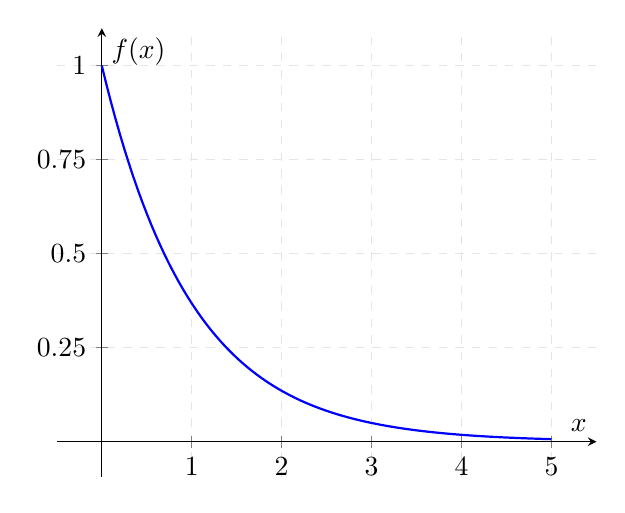
\begin{tikzpicture}
        \begin{axis}[
            domain=0:5,
            samples=100,
            axis x line=middle,
            axis y line=middle,
            xlabel={$x$},
            ylabel={$f(x)$},
            xtick={1,2,3,4,5},
            ytick={0.25, 0.5, 0.75,1},
            grid=major,
            grid style={dashed, gray!20},
            enlargelimits=true,
            %title={Exponential Distribution: $\lambda e^{-\lambda x}$ for $\lambda = 1$}
        ]
        \addplot[blue, thick] {exp(-x)};
        \end{axis}
    \end{tikzpicture}
    \source{ and processing: author}
\end{figure}

\begin{koment}
    Jak se exponencialni rozdeleni tyka BL? 

    Benfordovo rozdeleni muze pripominat exponencialni rozdeleni, proto bych mela popsat, jak to rozdeleni vypada, nakreslit nejaky pekny grafik a popsat co dela parametr lambda. Mozna by se hodil nejaky pekny priklad pouziti? 

    Mozna me jeste napada, jestli sem nenapsat co je to rozdeleni, frekventisticka definice pravdepodobnosti (since pocitam relativni frekvence vyskytu cislic na dane pozici a prirovnavam to k pravdepodobnostem) 
\end{koment}

Kdyz porovname exponencialni rozdeleni a rozdeleni podle benfordova zakona, narazime na dve vyrazne odlisnosti 
Benforduv zakon je diskretni (relativni frekvence pro jednotlive cislice), exponencialni rozdeleni je spojite. Dal, Benforduv zakon ma vetsi tails (jestli se tomu da vubec tak rikat pro diskretni rozdeleni), zatimco exponencialni rozdeleni ma tails velmi male. Pri zvoleni parametru, aby si byla rozdeleni blizka, vidime, jak jsou si odlisna. 

\begin{figure}[h]
    \centering
    \caption{Porovnani BL a Exp(0.45)}
    \label{fig:Exp0.45aBL}
    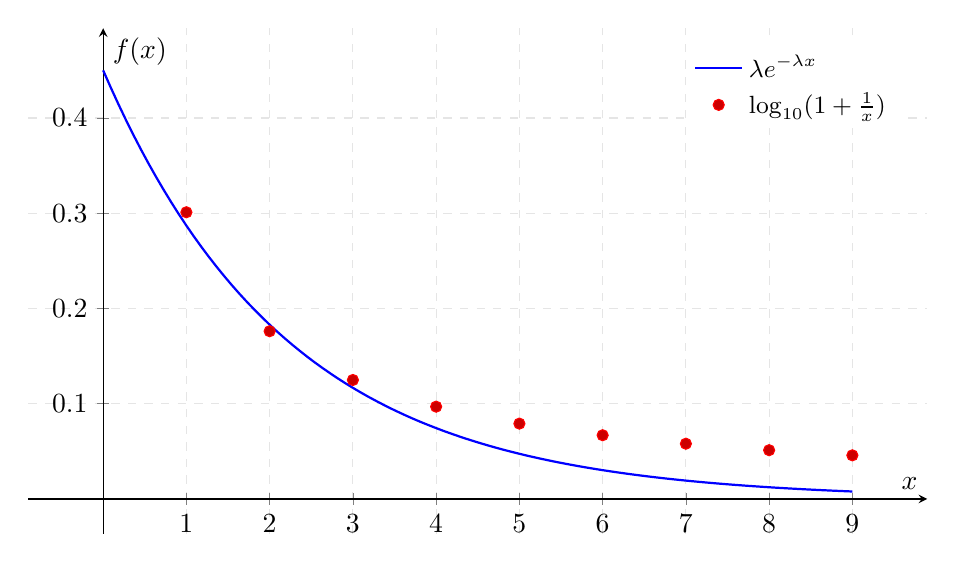
\begin{tikzpicture}
        \begin{axis}[
            width=13cm,  % Set the width of the plot
            height=8cm,  % Set the height of the plot
            domain=0:9,
            samples=100,
            axis x line=middle,
            axis y line=middle,
            xlabel={$x$},
            ylabel={$f(x)$},
            xtick={1,2,3,4,5,6,7,8,9},
            yticklabel style={/pgf/number format/.cd, fixed, precision=2}, 
            %ytick=\empty, 
            grid=major,
            grid style={dashed, gray!20},
            enlargelimits=true,
            %title={Porovnani BL a Exp(0.45)},
            legend style={draw=none, font=\small, cells={anchor=west}},
            legend pos=north east
        ]
        \addplot[blue, thick] {0.45*exp(-0.45*x)};
        \addlegendentry{$\lambda e^{-\lambda x}$}
        \addplot+[red, only marks, mark=*, mark size=2]
            coordinates {
            (1,0.3010) 
            (2,0.1761) 
            (3, 0.1249) 
            (4,0.0969) 
            (5,0.0791) 
            (6,0.0669) 
            (7,0.0580) 
            (8,0.0512) 
            (9,0.0458)
            };
        \addlegendentry{$\log_{10}(1 + \frac{1}{x})$}

        \end{axis}
    \end{tikzpicture}
    \source{ and processing: author}
\end{figure}


% %It is a non negative function, which sum equals to one. 

% For continuos variable is it defined as 

% \begin{equation}
%     P(x_1 \le X \le x_2) = \int\limits_{x_1}^{x_2} f (x) dx
% \end{equation}

% The distribution function is defined as 

% \begin{equation}
%     F(x) = P(X \le x), \quad \forall x \in R
% \end{equation}

% \begin{equation}
%     F(x) = \int\limits_{-\infty}^{x} f (t) dt, \quad -\infty <x<\infty
% \end{equation}

% \begin{koment}
%     neklesajici, v $-\infty$ je 0, v $\infty$ je 1

%     vymyslet jak to pojmout a propojit? 
% \end{koment}


\section{Hypothesis testing}

Hypothesis testing is a fundamental framework used to test a theory about a population based on a sample by comparing two hypotheses in statistics at the given \textbf{level of significance}. The tested hypothesis is the \textit{null hypothesis} $H_0$. An alternative to this, usually a negation, always a disjunction, is the \textit{alternative hypothesis} $H_1$. 

\begin{equation}
    H_0: \theta = \theta_0 \qquad \qquad H_1:  \theta \ne \theta_0
\end{equation}

In this case, we test whether the parameter $\theta$ is $\theta_0$ coming from a sample data. To test this assumption, a sample from the population is taken and analysed.  

Given the nature of the test, we select the \textbf{test statistic}. Its value comes from the sample of data and can fall into two sets. One, where its values are not in conflict with the null hypothesis, the acceptance region $V_\alpha$, and the other, where the values conflict with the null hypothesis, the \textbf{rejection region} $W_\alpha$. The \textbf{critical value} is the boundary for rejecting the null hypothesis. In the end, it is decided based on the critical value and test statistic which hypothesis is rejected, but neither accepted. Or the \textbf{p-value} is computed and compared to the level of significance. \cite{Mala2024, Marek2024}

\subsubsection*{Type I. and Type II. errors}

Working with sample data, there are two specific kinds of errors, and the probability of one influences the probability of the other. 

\textbf{Type I. error} $\alpha$ is the given level of significance, and it is the probability of rejecting the null hypothesis if the null hypothesis is correct. The $\alpha$ is usually set at 0.05. 

\begin{equation}
    \alpha = P(W_\alpha | H_0)
\end{equation}

\textbf{Type II. error} $\beta$ is the probability of not rejecting the null hypothesis if the null hypothesis is not correct. 

\begin{equation}
    \beta = P(V_\alpha | H_1)
\end{equation}

The probability $1-\beta$ is the \textbf{power of test} and denotes the probability of correct rejection of the null hypothesis. 

\subsubsection*{P-value}

The probability of obtaining a result which is as far or further from $H_{0}$ than the observed value. We reject the $H_{0}$ when  $p \le \alpha$ and we reject the $H_{1}$ when $p \ge \alpha$.

\subsection{$\chi^2$ goodness of fit test}

To check the compliance of the data to the BL, we can use the $\chi^2$ goodness of fit test. \\ This test is generally used to test whether the sample comes from an assumed population. The null hypothesis assumes the empirical distribution follows the theoretical distribution. The alternative hypothesis is the opposite. 

\begin{equation}
\begin{aligned}
    H_0&: \pi_d = p_d, \qquad d \in D\\
    H_1&: \pi_d \ne p_d
\end{aligned}
\end{equation}

$d$ comes from a set $D$, which contains all possible digits. For testing of the compliance of the first leading digits in numbers according to BL, $D = \{1,2,\dots,9\}$. $k$ is the number of digits, in this case $k = 9$.

The test statistic is given as such  

\begin{equation}
    \label{chi-sq-test}
    G= n \sum\limits_{d=1}^{9} \frac{(p_d -\pi_d)^2}{\pi_d} \qquad \qquad  G \approx \chi^2(k-1) 
\end{equation}

\begin{align*}
    \text{where } &\pi_d \text{ is the theoretical frequency under BL distribution}, \\
    &p_d \text{ is the empirical frequency from the data} \\ 
    &n \text{ is the sample size, and} \\
    &d \text{ is the corresponding digit}
\end{align*} 

as recommended in \citeauthor{Hronova2023}, \citeyear{Hronova2023} and  \citeauthor{kossovsky2014benford}, \citeyear{kossovsky2014benford}. 

There is one assumption, and that is that the sample size is large enough.  
$n \cdot \pi_d > 5$ for all $d$ (as put differently, there is enough observations for each digit). The rejection region under the null hypothesis is 

\begin{equation}
    W_\alpha = \left( \chi^2; G \ge \chi^2_{1-\alpha}(k-1) \right) = (\chi^2_{1-\alpha}(9-1), \infty)
\end{equation}

for the distribution of the first leading digit.

The test can be summed up as the larger the fraction \ref{chi-sq-test}, the poorer the fit between the empirical and theoretical frequencies.

% \begin{koment}
%     Pozor na stanovení N při testování pomocí chisq testu.
%     Je tam důležité odlišit, co je skutečně ta reálná populace - uvádí na příkladu, že populace mohou být sales revenue za celé čtvrtletí (57 tisíc záznamů) - unique price list, unique products... ale třeba sales revenue z malého coffee shopu bude třeba k nějaké populaci přihodit - je zde možné testovat compliance a u toho velkého vzorku ne? Nevím, jestli to chápu dobře... 

%     Pokud ten dataset existuje sám o sobě in its unique fashion, je to potom comparison, ne compliance. Compliance to bude když testujeme (za použití statistického testu) nějaký náhodný výběr. (takže třeba hlasy jen pro jednoho z kandidátů?) 

%     Pak se dal ukazují Z testy (pro jednotlivá pozorování) a pak ChiSq test pro cele. Nakonec je pak jeste zajimava smerodnatna odchylka jako measure odlisnosti. 
% \end{koment}

% \subsubsection*{Z test}

% This test is performed individually on a particular digit/combination, however, the false positive error (type I) is more likely for the overall test of the chi-square.

% Null hypothesis: Data obeys Benford's Law in the context of the particular digit/combination. % this individual observation obeys the benfords law ? 

% \begin{equation}
%     \label{z_test}
%     Z_d = \frac{|P_o - P_e| - 1/2n}{\sqrt{(P_e(1-P_e)/n}}
% \end{equation}

% \begin{align*}
%     \text{where } &P_o \text{ is the observed frequency of the particular digit/combination}, \\
%     &P_e \text{ is the expected Benford proportion for the particular digit/combination, and} \\ 
%     &n \text{ is the sample size}
% \end{align*} 

% We reject the null hypothesis when the $Z_d$ value is larger than $Z$ with the level of significance, $\alpha$. $Z$ refers to the Standardized Normal Distribution, a Normal distribution with mean 0 and standard deviation 1. \cite{kossovsky2014benford}

% \begin{koment}
%     Ještě se rozhoduju, jestli se mi to k něčemu nebude hodit, tak to tu zatím nechávám.  
% \end{koment}

\newpage

\section{Analysis workflow}

The analysis workflow used in this thesis can be seen in the figure \ref{fig:analysis-workflow}.  Its elements will be commented on below. 

\begin{figure}[h]
    \centering
    \caption{Analysis workflow}
    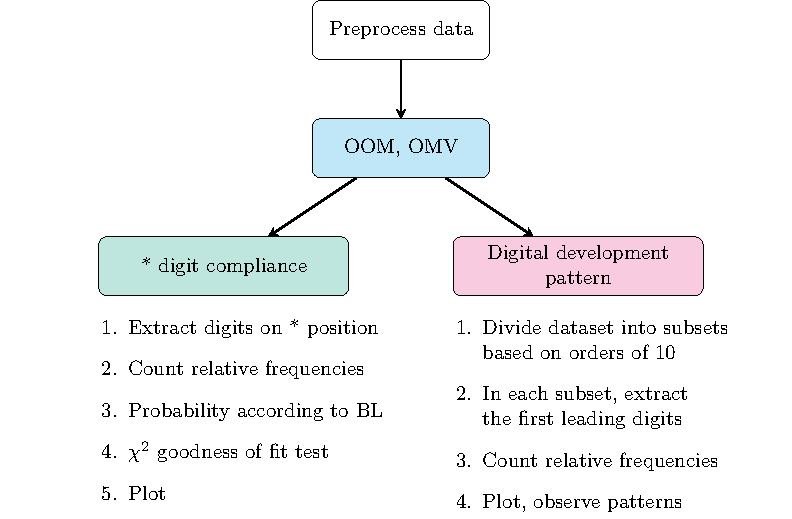
\includegraphics[width=0.9\linewidth]{BT-DT-eng/TemplateBT-DT/img/diagram.pdf}
    \label{fig:analysis-workflow}
    \source{ and processing: author}
\end{figure}

\subsubsection{Data preprocessing}

To start this process, the data is loaded into the R software. The election results for a small territory are chosen. One statistical unit is a town in the Czech Republic, a county in the USA or a polling station in Belarus. The decision for selection of the size of the region is based on individual accounting for the size of the country, total sample size and availability, so that the dataset would be suitable for the methodology of this thesis, namely the BL.

Next, the relevant variables are selected. Most important are the vote counts of the candidates and the totals. There are two candidates in the Czech elections, the USA and Belarus have two main candidates and a couple of other candidates with very few votes. The two candidates with the majority of votes are selected. 

Afterwards, the data types are changed into those that are suitable for the analysis; vote counts are typically a numerical discrete (integer) variable, and their validity is checked (control sums of the number of votes). 

\subsubsection{Order of Magnitude}

OOM measure tells us whether we can use the last digit test responsibly. If the OOM test is rejected ($OOM < 3$), we should not test compliance of the last digits or last two digits to the uniform distribution (which is the generalised BL). The relative frequencies are influenced by their position. So instead of last digits, we should take their position from the most significant digit - \_. leading digit. 

\subsubsection{Digit compliance on a given position} 

In this first and most important section, we look at how well the relative frequencies follow the BL variation. Namely, we shall focus on these positions in numbers: 

\begin{itemize}
    \item First digit 
    \item First two digits 
    \item Second digit 
    \item Third digit 
    \item Last digit
\end{itemize}

In the first digit distribution, the most famous BL is applied, as formulated in \ref{BZ-general_first} equation. The same information, but in better detail, is seen in the distribution of the first two digits. The second digit distribution, as noted by \citeauthor{Beber2012} and \citeauthor{Mebane2011}, is suitable for detecting digital fraud. Similarly, with the third digit distribution, for which the distribution starts to resemble the uniform distribution, as can be seen on \ref{fig:third-digit-law} graph. And lastly, we shall take a look at the relative frequencies of the last digits.

Firstly, the relevant digits on the given position need to be extracted. Then their relative frequency and the probability according to the BL are counted, as seen in an example table \ref{table:BL-table}. This table is used for the following testing and plotting.  

\begin{table}[h]
\centering
    \caption{The frequencies of the first leading digits and probabilities according to the BL \\the Czech presidential elections 2023}
    \begin{tabular}{c|rrrcr}
        \hline
        digit & Freq & Total & RelFreq & BL     & diff    \\ \hline
        1     & 1866 & 6320  & 0.2953  & 0.3010 & -0.0058 \\
        2     & 1090 & 6320  & 0.1725  & 0.1761 & -0.0036 \\
        3     & 811  & 6320  & 0.1283  & 0.1249 & 0.0034  \\
        4     & 621  & 6320  & 0.0983  & 0.0969 & 0.0013  \\
        5     & 492  & 6320  & 0.0778  & 0.0792 & -0.0013 \\
        6     & 434  & 6320  & 0.0687  & 0.0669 & 0.0017  \\
        7     & 368  & 6320  & 0.0582  & 0.0580 & 0.0002  \\
        8     & 302  & 6320  & 0.0478  & 0.0512 & -0.0034 \\
        9     & 336  & 6320  & 0.0532  & 0.0458 & 0.0074  \\ \hline
    \end{tabular}
    \source{: \citeauthor{CR23data}, \citeyear{CR23data}, processing: author}
    \label{table:BL-table}
\end{table}

All those distributions for given positions shall be tested by the $\chi^2$ goodness of fit test, as defined in \ref{chi-sq-test}, and then plotted with the corresponding p-value of the test. In some graphs, the p-value is labelled as unreliable, which signifies that the assumption of the test was not met (the absolute frequency of any digit was smaller than 5). 

There are also two points of view, the first on the totals of votes and the second on the dual plots with the counts for the individual candidates. This is important to see if there was an interest in manipulating one candidate more than the other. 

The distribution of the last two digits is not examined due to inconclusive results given by the nature of the data - the range is from 0 to 10000 usually, depending on the country and the examined regional level, and for some numbers the last two digits can be the whole number, so the relative frequencies do not match. 

\subsubsection{Digital development pattern} 

In this part, an accompanied indicator is examined, the digital development pattern. The expected behaviour of such is described in \ref{DDPattern}. It is not so strict; we are searching for some anomalies while also observing what part of the dataset is represented in a given range. This provides additional information on how well the data would comply with the BL. 

% \subsubsection{Correlation between selected variables}

% As \citeauthor{Lebeda2021} mentioned in their paper, observing the relationships between the valid votes and the votes for each candidate is an essential part of election analysis, so this part shall not be forgotten. It is not in the primary focus of this thesis, however, it will add a point of view in this analysis. The results from this part are just for a general picture. 

% We are searching for some patterns, a high correlation between turnout and votes for a specific candidate, or any anomalies of other kinds. Ideally, the turnout, the percentage of valid votes, should both be uncorrelated, unrelated to the share of votes of each candidate, as \citeauthor{Lebeda2021} mentioned. 
